%%================================================
%% Appendix H
%%================================================
\chapter[แบบสอบถามประเมินความพึงพอใจ Google Form]{\texorpdfstring{ภาคผนวก ซ\\แบบสอบถามประเมินความพึงพอใจ Google Form}{Appendix H: Google Form Questionnaire}}
\label{app:legacy_google_form}

ภาคผนวกนี้รวบรวมภาพหน้าจอจากแบบสอบถาม Google Form ที่ใช้เป็นหลักฐานประกอบการเก็บความคิดเห็นและความพึงพอใจของผู้ใช้งานหรือผู้ดูแลในช่วงการประเมินระบบต้นแบบ ภาพในภาคผนวกนี้นำมาจากชุดเอกสารเดิมโดยคัดลอกเข้ามาไว้ในโฟลเดอร์ของเล่มปัจจุบันเพื่อให้สามารถ compile ได้โดยไม่อ้าง path ภายนอก

\begin{figure}[!htbp]
    \centering
    \begin{subfigure}[t]{0.47\textwidth}
        \centering
        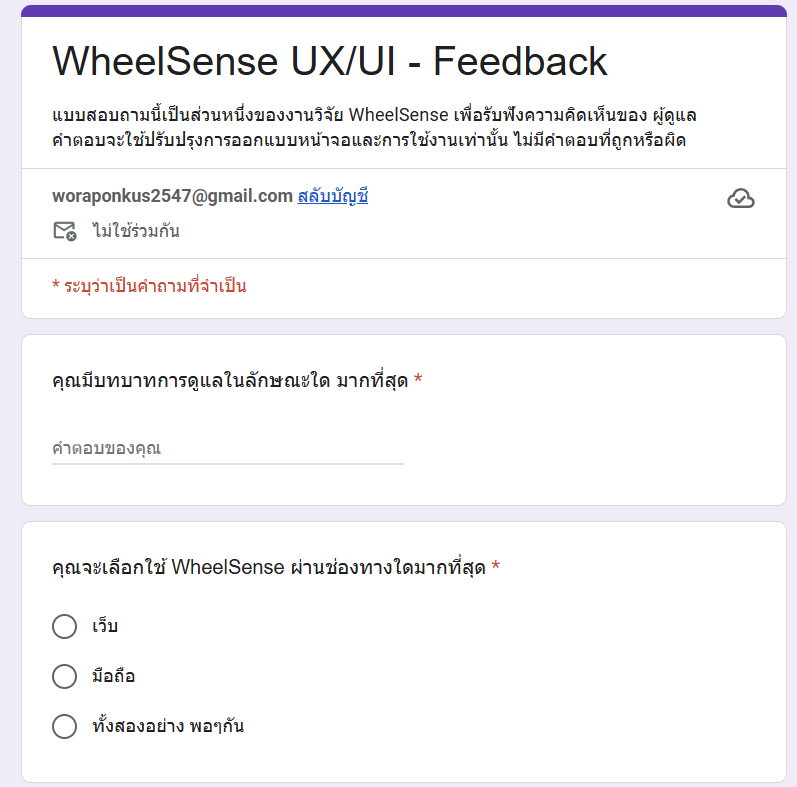
\includegraphics[width=\linewidth,height=0.38\textheight,keepaspectratio]{assets/appendices/legacy-google-form/form1.png}
        \caption{หน้าแรกและคำชี้แจง}
        \label{fig:appH_form1}
    \end{subfigure}
    \hfill
    \begin{subfigure}[t]{0.47\textwidth}
        \centering
        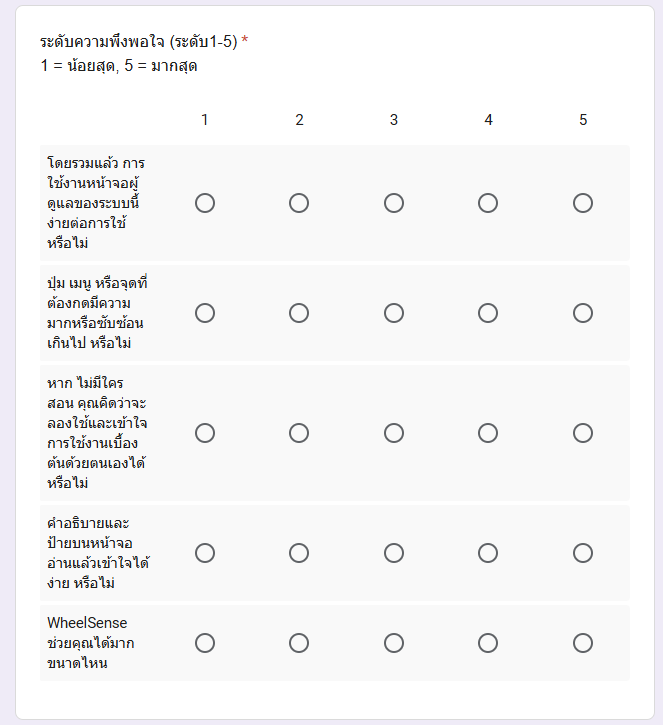
\includegraphics[width=\linewidth,height=0.38\textheight,keepaspectratio]{assets/appendices/legacy-google-form/form2.png}
        \caption{ส่วนคำถามประเมินความพึงพอใจ}
        \label{fig:appH_form2}
    \end{subfigure}
    \caption{ตัวอย่างหน้าจอแบบสอบถามประเมินความพึงพอใจส่วนต้น}
\end{figure}

\begin{figure}[!htbp]
    \centering
    \begin{subfigure}[t]{0.47\textwidth}
        \centering
        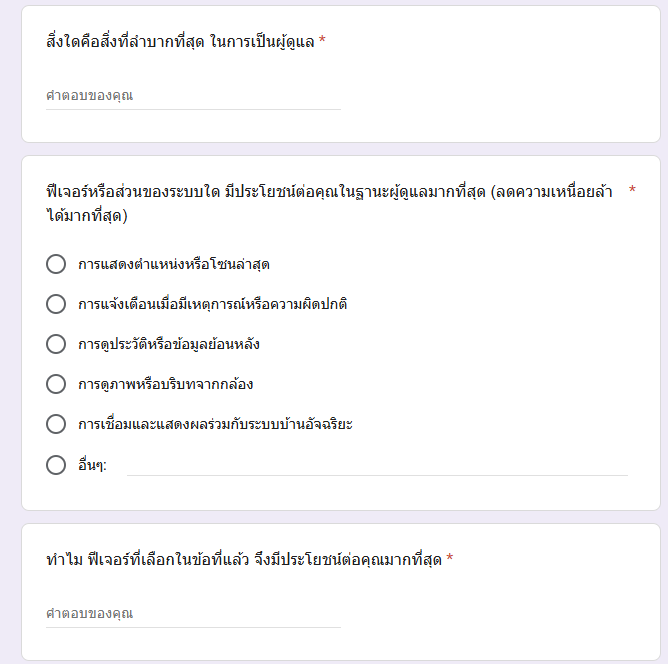
\includegraphics[width=\linewidth,height=0.38\textheight,keepaspectratio]{assets/appendices/legacy-google-form/form3.png}
        \caption{ส่วนคำถามเพิ่มเติม}
        \label{fig:appH_form3}
    \end{subfigure}
    \hfill
    \begin{subfigure}[t]{0.47\textwidth}
        \centering
        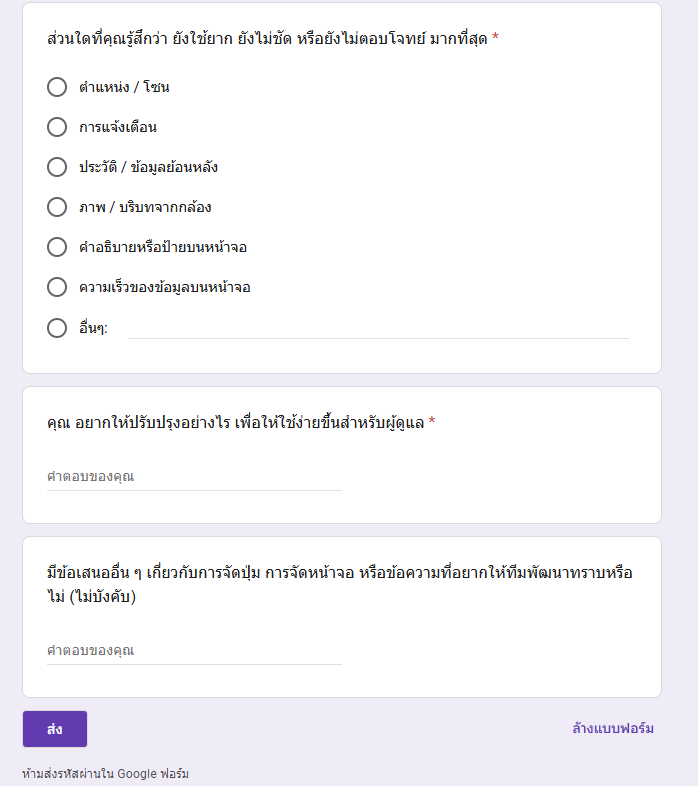
\includegraphics[width=\linewidth,height=0.38\textheight,keepaspectratio]{assets/appendices/legacy-google-form/form4.png}
        \caption{ข้อเสนอแนะและหน้าขอบคุณ}
        \label{fig:appH_form4}
    \end{subfigure}
    \caption{ตัวอย่างหน้าจอแบบสอบถามประเมินความพึงพอใจส่วนท้าย}
\end{figure}
